\setcounter{chapter}{8}
\setcounter{section}{1}
\setcounter{question}{0}
\setcounter{hint}{0} % Only for first assignment in chapter

%%%%%%%%%%%%%%%%%%%%%%%%%%%%%%%%%%%%%%%%%%%%%%%%%%%%%%%%%%%%%%%%%%%%%%%%%%%
% Assignment 8.1: Specifying and interpreting a prior distribution
%%%%%%%%%%%%%%%%%%%%%%%%%%%%%%%%%%%%%%%%%%%%%%%%%%%%%%%%%%%%%%%%%%%%%%%%%%%

\rassignment{Specifying and interpreting a prior distribution}

In this final chapter, we stray away from the traditional statistical methods that you have learned (\concept{confidence intervals} and \concept{p-values}), and introduce a different methodology; Bayesian statistics. Bayesian statistics expresses the most basic idea in learning, namely, that your prior belief in an event is updated after observing data to a posterior belief. By first specifying your prior beliefs, you allow yourself to learn from the data that you have collected, thereby updating your prior belief to a more informed posterior belief. Bayesian statistics is a powerful tool and can help you to update your existing beliefs in the context of new business information. \\

In Bayesian inference your prior beliefs about a \concept{parameter} are expressed through a \concept{probability distribution}. For example, in tossing a coin, the probability of heads occurring may be defined as a \concept{parameter} denoted by $\theta$. Your initial probability distribution (i.e., beliefs) on $\theta$ is called the \concept{prior distribution} and can be interpreted quite visually. The figure below shows three possible prior distributions for the probability of heads in a coin toss. The area under the curve represents probability.

\begin{center}
    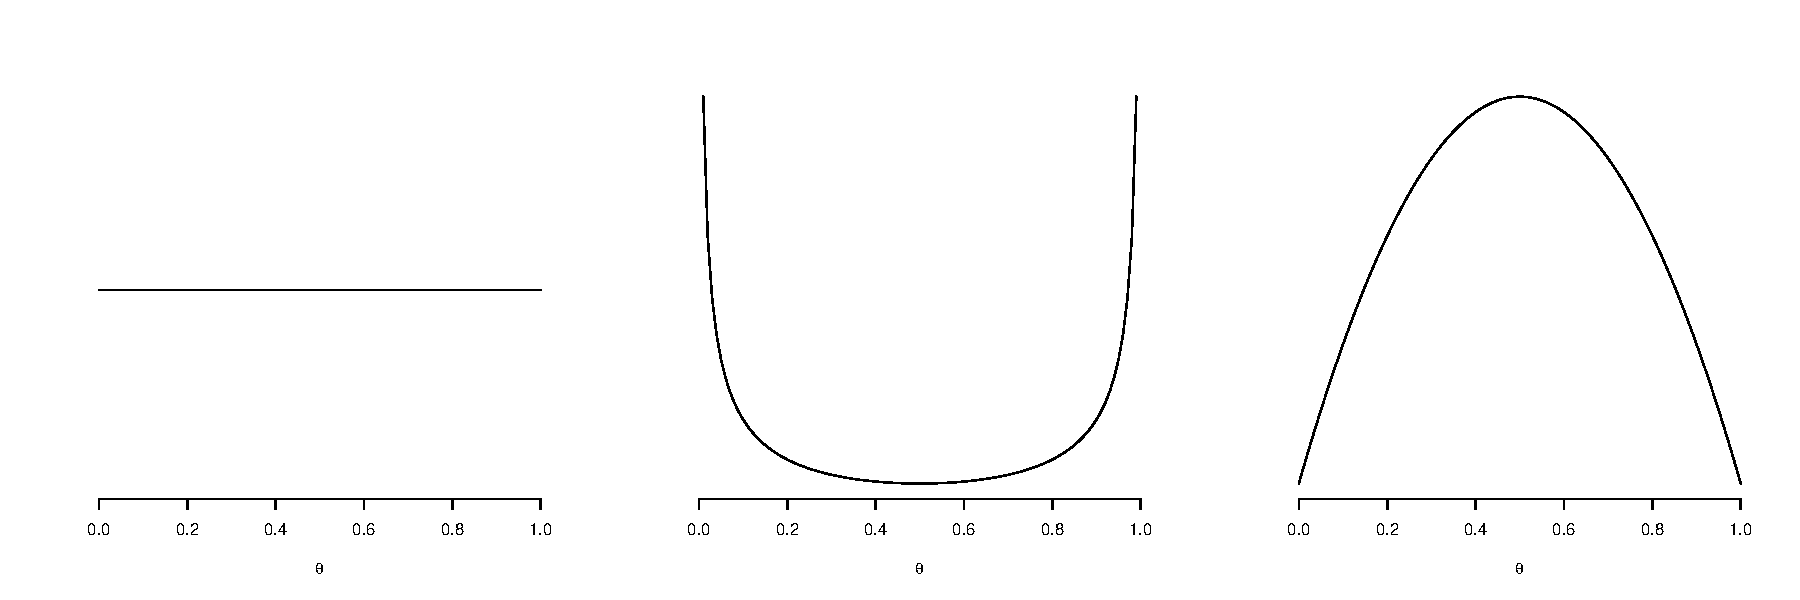
\includegraphics[width=\textwidth]{Files/Images/priorDistributions.pdf}
\end{center}

\question{
    Interpret the three \concept{prior distributions} above and discuss what information about the probability of the coin occurring on heads $\theta$ they incorporate.
}

\twolineanswerbox

\clearpage % Page break

When estimating a proportion (like the probability of head in a coin toss) you can use the common $Beta(\alpha,\, \beta)$ distribution as a prior distribution on $\theta$ since it is restricted to be within the range of zero to one. The $Beta(\alpha,\, \beta)$ distribution has two parameters, $\alpha$ and $\beta$, that have an effect on its shape. By playing around with these values, you can create the \concept{prior distribution} that reflects your beliefs as accurately as possible. \\

Run the following code in \texttt{R} to create the \concept{prior distribution} that is displayed on the left of the figure: \\

\codeblock{alpha <- 1 \\
beta <- 1 \\
curve(dbeta(x, alpha, beta), xlab = expression(theta), ylab = \textquotesingle\textquotesingle, yaxt = \textquotesingle n\textquotesingle)}

\question{Recreate the middle and right \concept{prior distributions} by changing the values for \rcode{alpha} and \rcode{beta} and running the code again. What are the values of $\alpha$ and $\beta$ for these distributions?}

\rcodeanswersmall

\emptyanswerbox{
    Middle: \hspace*{5cm} Right \\
    \\
    $\alpha$: \shortanswerline  \hspace*{2.5cm} $\alpha$: \shortanswerline
    \answerbreak
    $\beta$: \shortanswerline \hspace*{2.5cm} $\beta$: \shortanswerline
}

\question{How would you draw a \concept{prior distribution} for $\theta$ if you believed the coin was definitely biased towards heads? And for one that is biased towards tails? Draw your \concept{prior distributions} below.}

\emptyanswerbox{
    \vspace*{-.5cm}
    \hspace*{2.1cm} Biased towards heads: \hspace*{0.65cm} Biased towards tails:
    \vspace*{-7.5pt}
    \begin{center}
        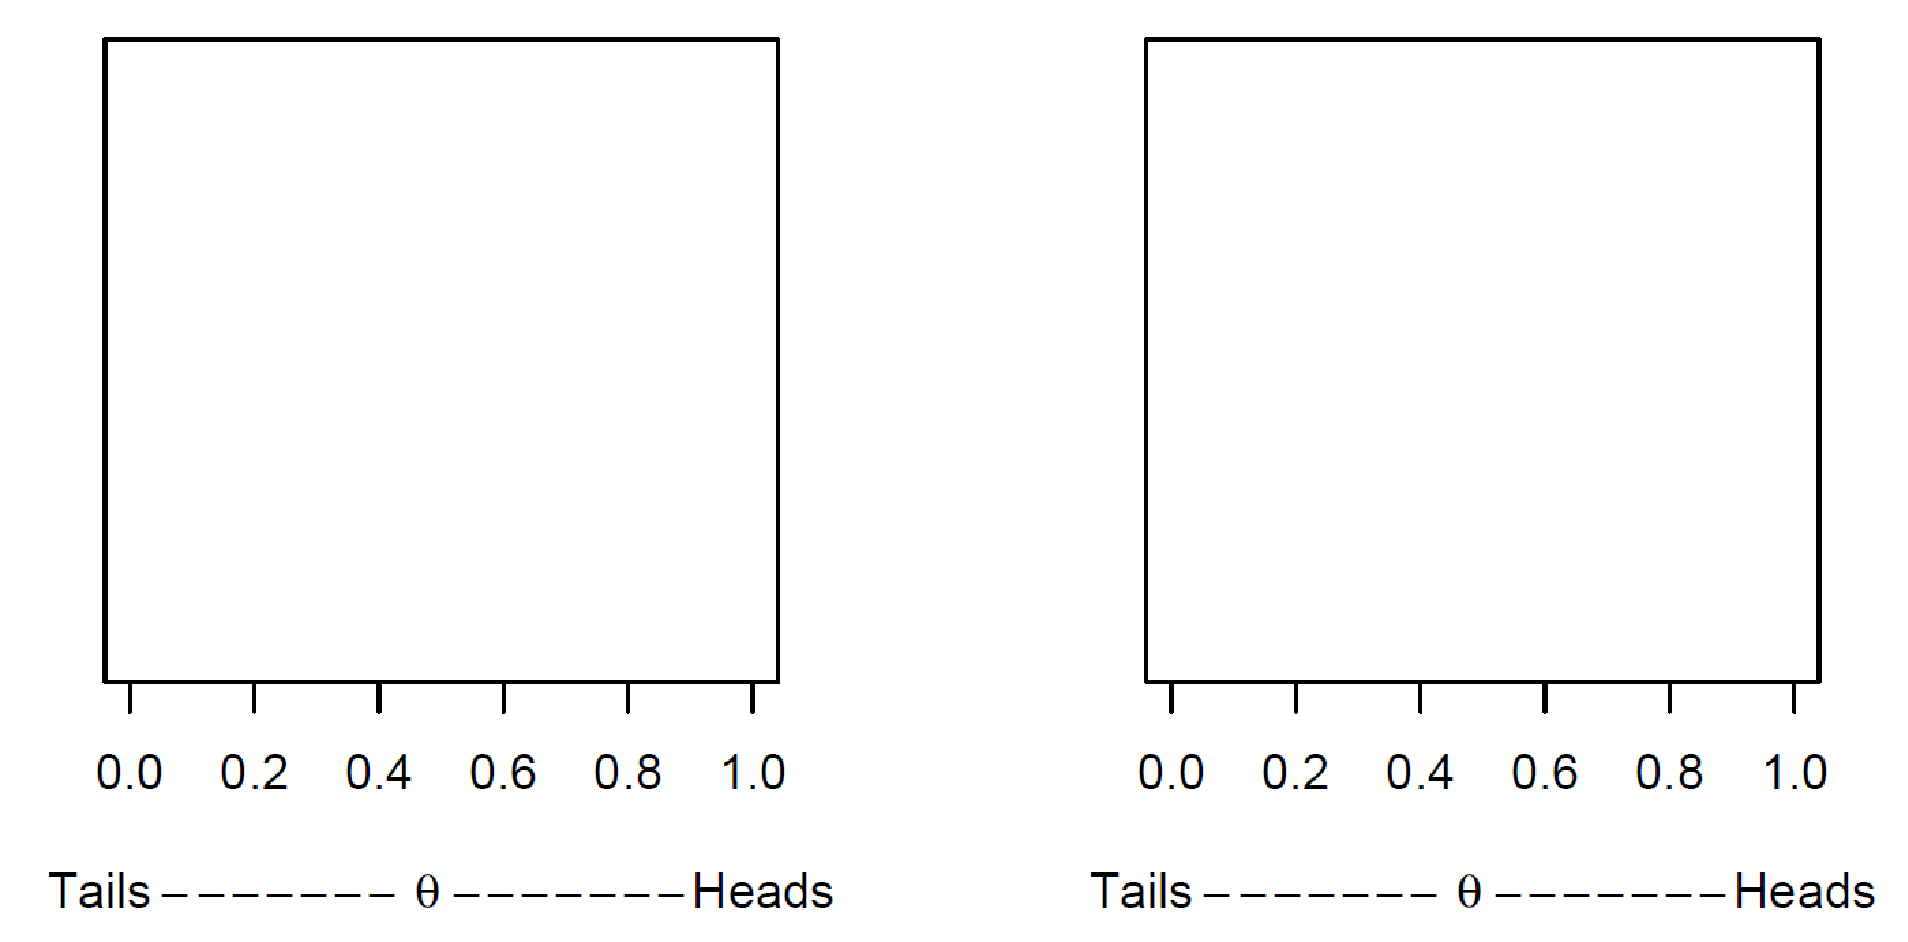
\includegraphics[height=5.3cm]{Files/Images/priorDistributionsAnswerField.pdf}
    \end{center}
}

\clearpage % Page break